% !TeX program = xelatex
% English CV of Yi Shouzhuo.
% Template identical to CV_cn.tex (WHU grey-bar headings, logo & photo header);
% only the text is translated. Compile with xelatex (two passes):
%   xelatex -interaction=nonstopmode CV.tex
%   xelatex -interaction=nonstopmode CV.tex
% build.py 还会自动编译并发布到 content/CV/CV-PDF-en.pdf。
\documentclass[10pt,article]{article}
\usepackage{pdfpages}
\usepackage[letterpaper,margin=0.3in]{geometry}
\usepackage{graphicx}
\usepackage{booktabs}
\usepackage{url}
\usepackage{enumitem}
\usepackage{palatino}
\usepackage{tabularx}
\fontfamily{SansSerif}
\selectfont

\usepackage[UTF8]{ctex}
\usepackage[T1]{fontenc}
\usepackage
%[ansinew]
[utf8]
{inputenc}

\usepackage{color}
\definecolor{mygrey}{gray}{0.82}
\textheight=9.75in
\raggedbottom

\setlength{\tabcolsep}{0in}
\newcommand{\isep}{-2 pt}
\newcommand{\lsep}{-0.5cm}
\newcommand{\psep}{-0.6cm}
\renewcommand{\labelitemii}{$\circ$}

\pagestyle{empty}
%-----------------------------------------------------------
%Custom commands
\newcommand{\resitem}[1]{\item #1 \vspace{-2pt}}
\newcommand{\resheading}[1]{{\small \colorbox{mygrey} { \begin{minipage}{0.99\textwidth}\centering{\textbf{#1 \vphantom{p\^{E}}}}\end{minipage}}}}
\newcommand{\ressubheading}[3]{
	\begin{tabular*}{6.62in}{l @{\extracolsep{\fill}} r}
		\textsc{{\textbf{#1}}} & \rightline\textsc{\textit{[#2]}} \\
	\end{tabular*}\vspace{-8pt}}
%-----------------------------------------------------------

\begin{document}

	\begin{table}[h]
		\begin{minipage}{0\linewidth}
			\centering
			
\includegraphics[height =0.8in]{./whulogo.png}
		\end{minipage}
		\begin{minipage}{0.9\linewidth}
			%\centering
			% 保持模板的 70pt 列距；学校信息拆成两行让第一列变短，
			% 联系列就不会像单行长英文那样被挤出页边
			\setlength{\tabcolsep}{70pt}
			\def\arraystretch{1.1}
			\begin{tabular}{ll}
				\textbf{\Large{Yi Shouzhuo}}  &  {Mobile: +86 13667280239} \\
				\textbf{School of Computer Science} &  {Email: yishouzhuo@whu.edu.cn} \\
				\textbf{Hongyi Honor Class} &   \\
				\textbf{Wuhan University}
			\end{tabular}
		\end{minipage}
		\begin{minipage}{0\linewidth}
			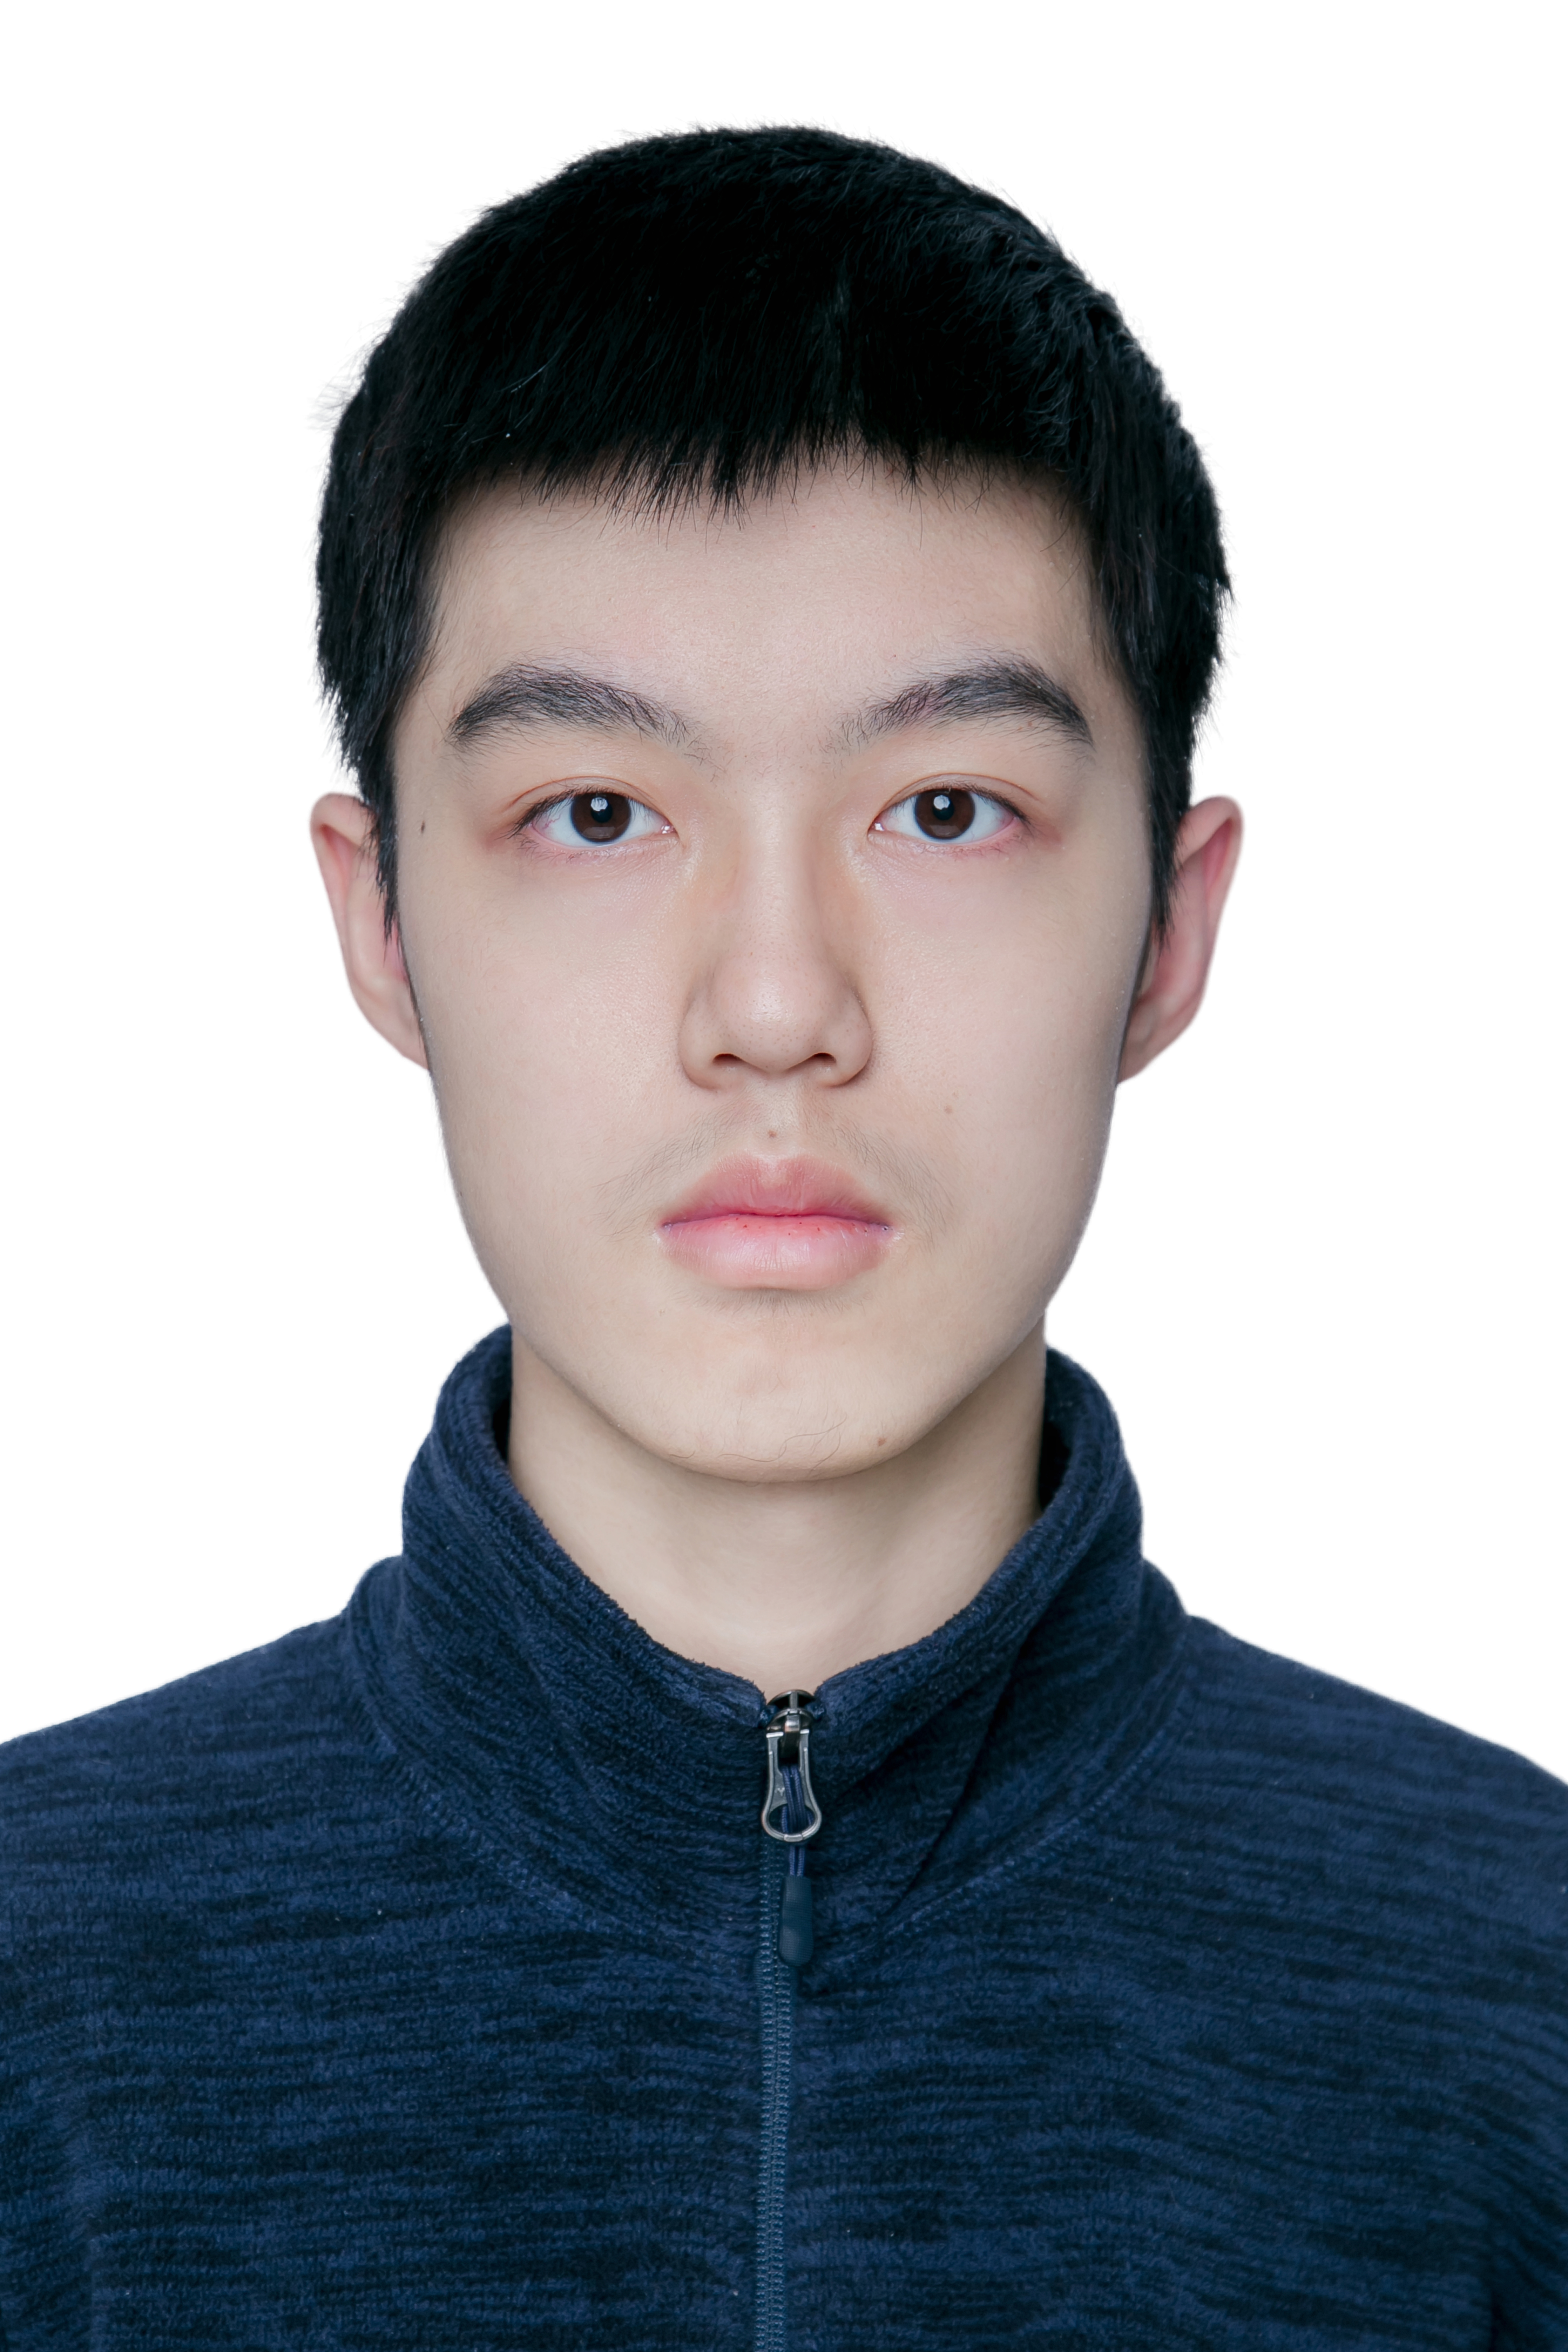
\includegraphics[height =1in]{photo.png}
		\end{minipage}\hfill
	\end{table}

	\noindent
	\resheading{\textbf{Education}}\\[-0.5cm]
	\begin{itemize}
		\setlength\itemsep{-0.45em}
		\item Major: Computer Science and Technology (Hongyi Honor Class) \hfill {[2024 - 2028]}
		\\GPA: 3.87/4.00 (5/29)
		\\Average: 92.65/100 (5/29)
		\\CET-4: 608 \quad CET-6: 557
		\\Courses and grades: Advanced Programming Language A (97), Data Structures A (97), Computer Organization and Architecture A (85), Operating Systems A (91), Algorithm Design and Analysis (96)
		\\[-0.6cm]
	\end{itemize}


	\noindent
	\resheading{\textbf{Research Experience}}\\[-0.45cm]
	\begin{itemize}
		\setlength\itemsep{-0.2em}

		\item \textbf{SIGMA, Wuhan University}\hfill {[Jan. 2025 - Jul. 2025]}
		\begin{itemize}[noitemsep,nolistsep]
			\item Advisor: Dr. Lvyang Tong (Postdoctoral Researcher, WHU)
			\item Program: Student Innovation and Entrepreneurship Training Program
			\item Research: Multimodal interpretable models for fetal congenital heart disease
			\item Output: The provincial-level project was successfully concluded
		\end{itemize}

		\item \textbf{SIGMA, Wuhan University}\hfill {[Sep. 2025 - Jul. 2026]}
		\begin{itemize}[noitemsep,nolistsep]
			\item Advisor: Assoc. Prof. Youfa Liu (School of Computer Science, WHU)
			\item Research: Source-free domain adaptation based on large vision--language models
			\item Output: One paper in preparation
		\end{itemize}
        \item \textbf{ARTE Group, University of Chinese Academy of Sciences}\hfill\mbox{[Jul. 2026 - Present]}
		\begin{itemize}[noitemsep,nolistsep]
			\item Advisor: Prof. Tong Zhang (Tenure-track Assistant Professor, UCAS)
			\item Research: World models
		\end{itemize}

	\end{itemize}
	\noindent
	\resheading{\textbf{Project Experience}}\\[-0.45cm]
	\begin{itemize}
		\setlength\itemsep{-0.2em}


		\item \textbf{ByteDance Engineering Bootcamp --- Story-to-Video}\hfill {[Dec. 2025]}
		\begin{itemize}[noitemsep,nolistsep]
			\item Built the full pipeline from natural-text input to video output: visual storyboard management, per-shot editing, and integrated image generation, dynamic video rendering, and AI-powered voiceover
			\item Contributed to the deployment of backend models (LLM/TTS) and the design of the communication links between the backend and the server
			\item Successfully completed the ByteDance Engineering Bootcamp
		\end{itemize}

	\end{itemize}

	\noindent
	\resheading{\textbf{Skills
			%	\& Research Interests
	}}\\[-0.5cm]
	\begin{itemize}
		\item Proficient in Python/PyTorch; early research training has built up the ability to take an idea from concept to code, experiments, and parameter tuning\\[-0.7cm]
		\item Familiar with the essential tooling: ssh/\LaTeX\\[-0.7cm]
	\end{itemize}


	\noindent
	\resheading{\textbf{Awards and Honors}}\\[-0.2cm]
	\begin{itemize}[noitemsep,nolistsep]

		\item \textbf{2026 Lei Jun Scholarship for Undergraduate Students in Computer Science}\hfill\quad\mbox{[University]}\\[-0.4cm]



		\item \textbf{2024-2025 16th Blue Bridge Cup, C/C++ --- Second Prize}\hfill\quad\mbox{[Provincial]}\\[-0.4cm]

		% \item \textbf{2024-2025 17th Huazhong Cup Mathematical Modeling Challenge for College Students --- Second Prize}\hfill\quad\mbox{[Provincial]}\\[-0.4cm]



		\item \textbf{2025-2026 National College Mathematics Competition, Non-Mathematics Track A --- Second Prize}\hfill\quad\mbox{[Provincial]}\\[-0.4cm]

		\item \textbf{2025-2026 2nd CCF Algorithm Capability Contest --- Second Prize }\hfill\quad\mbox{[Provincial]}\\[-0.4cm]
		\item \textbf{2025-2026 Group Programming Ladder Tournament (GPLT) --- National Third Prize}\hfill\quad\mbox{[National]}\\[-0.4cm]
		\item \textbf{2026 National Collegiate Computer Systems Capability Contest --- Operating System Design Contest, OS Kernel Implementation Track --- National Second Prize}\hfill\quad\mbox{[National]}\\[-0.4cm]

	\end{itemize}


	\noindent
	\resheading{\textbf{Self Assessment}}\\[-0.2cm]
	\begin{itemize}[noitemsep,nolistsep]
		\item{\textbf{Strong mathematical understanding and solid theoretical learning ability; self-motivated and quick to adapt; eager to turn understanding into practical contributions in challenging research and to prove my capability as a researcher}}\\[-0.4cm]
	\end{itemize}

	%\includepdf[pages=1]{GPA大二下.pdf}
\end{document}
